\section{Magnetic Levitation System}
\label{sec:magnetic_levitation_system}

As stated in the introduction, the system under study is the \acrfull{mls} provided by \texttt{Inteco} (product vebsite: \url{https://www.inteco.com.pl/products/magnetic-levitation-systems/}).
In Figure \ref{fig:MLS} a picture of the system present in the laboratory is shown.

\begin{figure}[H]
    \centering
    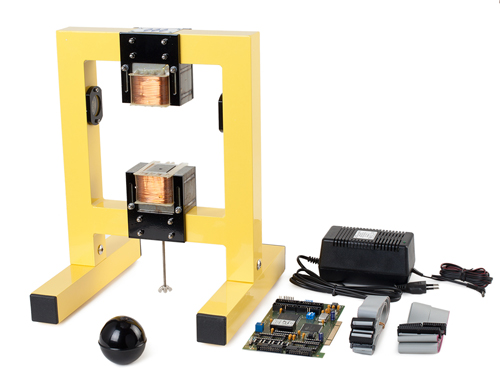
\includegraphics[width=0.7\textwidth]{./img/maglev_picture.jpg}
    \caption{\acrlong{mls}}
    \label{fig:MLS}
\end{figure}

As it can be seen quite clearly, the system is composed of a simple mechanical structure that is used to support two electromagnets and an optical infrared sensor.
Along with the mechanical structure, a ferromagnetic ball and a control unit are present.

At its core principle, the system uses the interaction between the magnetic field generated by the electromagnets and the ferromagnetic ball to keep the ball in a desired position.
The optical sensor is used to measure the position of the ball and provide feedback to the control unit that, in turn, adjusts the current flowing through the electromagnets to keep the ball in a desired position.
In Figure \ref{fig:MLS_schematic} a schematic representation of the upper half of the system is shown.

\begin{figure}[H]
    \centering
    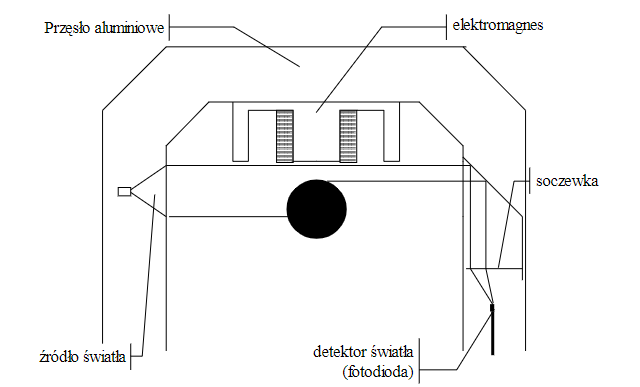
\includegraphics[width=0.5\textwidth]{./img/maglev_scheme.png}
    \caption{Schematic representation of the \acrshort{mls} system.}
    \label{fig:MLS_schematic}
\end{figure}

\paragraph{Real world application}

Despiste the fact that our system is a simplified version of a real-world application, the magnetic levitation principle is used in many real-world applications.

One of the most common applications is the magnetic levitation trains, also known as `MagLev' trains.
These trains use the magnetic levitation principle to lift the train off the tracks and propel it forward using the magnetic field generated by the tracks.
The main advantage of this technology is the absence of friction between the train and the tracks, which allows the train to reach higher speeds and reduce the noise characteristic of the traditional trains.
Some of the fastest (operating) trains in the world are MagLev trains, with the Shanghai MagLev train being the fastest, reaching a top speed of $623 km/h$ \cite{WikiSCMaglev}.

Another application of the magnetic levitation principle is the magnetic bearings.
These bearings use the magnetic field generated by electromagnets to levitate a rotor and keep it in a desired position.
The main advantage of this technology is the absence of mechanical contact between the rotor and the stator, which allows the rotor to reach higher speeds and reduce the wear of the components.

\subsection{Model derivation}
\label{subsec:model_derivation}

The \acrshort{mls} is a complex system that can be divided into two main subsystems:

\begin{itemize}
    \item \textbf{Electromagnetic subsystem}: it takes into account the electrical components of the system from the power supply to the generation of the magnetic field by the coils;
    \item \textbf{Mechanical subsystem}: it takes into account the dynamics of the ball and all the forces acting on it, including the electromagnetic forces generated by the magnetic field.
\end{itemize}

Due to the presence of the ball that moves inside a magnetic field, a complex connection between the two subsystems that goes beyond the simple force balance exists.
For this reason, it's almost impossible to derive a complete model without considering both subsystems at the same time.

In Figure \ref{fig:system_model}, a schematic representation of all the components and forces acting on the system is shown.
Instead, in Table \ref{tab:components} a brief description of the components of the system and their units is reported.

\begin{figure}[H]

    \begin{minipage}{0.40\textwidth}

        \centering

        \begin{tikzpicture}[european voltages]

            \def\radius{0.3}

            % Upper circuit
            \node at (-1.0, 3.5) {$T_1$};
            \draw (-3, 3.5) node [right] {$+$}
            to [short] ++(0, -1)
            to [R, l^=$R_1$, resistors/zigs=6] ++(2, 0)
            to [variable cute inductor, i>^=$I_1$, l=$L_1$] ++(2, 0)
            to [short] ++(0, +1) node [right] {$-$};

            % Reference system
            \draw[|->] (-1.0, +2.5) -- ++(0, -3) node[left] {$z$, $\dot{z}$, $\ddot{z}$};

            % Ball
            \filldraw[fill=gray, draw=black] (0, 0) circle (\radius);

            % Upward forces
            \draw[thick, ->] (-0.1, +\radius) -- ++(0, +1.5) node[right] {$F_{\text{em1}}$};
            \draw[thick, ->] (+0.0, +\radius) -- ++(0, +1.0) node[right] {$F_{\text{in}}$};
            \draw[thick, ->] (+0.1, +\radius) -- ++(0, +0.5) node[right] {$F_{\text{d}}$};

            % Downward forces
            \draw[thick, ->] (+0.1, -\radius) -- ++(0, -0.5) node[right] {$F_{\text{g}}$};
            \draw[thick, ->] (-0.1, -\radius) -- ++(0, -1.0) node[right] {$F_{\text{em2}}$};

            % Lower circuit
            \node at (-1.0, -3.0) {$T_2$};
            \draw (-3, -3) node [right] {$+$}
            to [short] ++(0, +1)
            to [R, l_=$R_2$, resistors/zigs=6] ++(2, 0)
            to [variable cute inductor, i>_=$I_2$, l_=$L_2$] ++(2, 0)
            to [short] ++(0, -1) node [right] {$-$};

        \end{tikzpicture}

    \end{minipage}
    %
    \hfill
    %
    \begin{minipage}{0.55\textwidth}

        \centering

        \begin{tabular}{|c|l|c|}
            \hline
            \textbf{Name}      & \textbf{Description}             & \textbf{Units} \\
            \hline
            $F_{\text{g}}$     & Gravitational force              & N              \\
            $F_{\text{in}}$    & Inertial force                   & N              \\
            $F_{\text{d}}$     & Drag force                       & N              \\
            $F_{\text{em1,2}}$ & Electromagnetic force            & N              \\
            $R_{1,2}$          & Resistance of the coil           & $\Omega$       \\
            $L_{1,2}$          & Inductance of the coil           & H              \\
            $I_{1,2}$          & Current flowing through the coil & A              \\
            $V_{1,2}$          & Voltage applied to the coil      & V              \\
            $T_{1,2}$          & Temperature of the coil          & $^\circ C$     \\
            \hline
        \end{tabular}

    \end{minipage}

    \caption{Schematic representation of the \acrshort{mls} system and description of the components.}
    \label{fig:system_model}
    \label{tab:components}

\end{figure}


In the following sections, we will derive the equations that governs the \acrshort{mls} system, adopting an energetic approach that starts from the energy conservation principle.

\subsubsection{Mathematical model}
\label{subsubsec:mathematical_model}

We can now proceed with the derivation of the equations that govern the system.

At first, we can recall that the energy conservation principle states that the sum of the kinetic, potential, and dissipated energy of the system is equivalent to the work done by the external forces acting on the system.

\paragraph{Lagrange's equation}

Thanks to the Lagrange's equation we write the following, that encaptulates the energy conservation principle:

\begin{equation}
    \frac{d}{dt} \left( \frac{\partial \mathcal{T}}{\partial \dot{\mathbf{u}}} \right) - \frac{\partial \mathcal{T}}{\partial \mathbf{u}} + \frac{\partial \mathcal{D}}{\partial \dot{\mathbf{u}}} + \frac{\partial \mathcal{U}}{\partial \mathbf{u}} = \mathcal{Q}
    \label{eq:lagrange_equation}
\end{equation}

Where $\mathbf{u}$ is the generalized coordinates of the system, $\mathbf{T}$ is the kinetic energy of the system, $\mathbf{D}$ is the dissipated energy of the system, $\mathbf{U}$ is the potential energy of the system, and $\mathbf{Q}$ is the generalized input to the system.

At first, we can give a definition of all the energetic terms included in Equation \ref{eq:lagrange_equation} for the \acrshort{mls} system.
Notice that with respect to traditional purely mechanical systems, we also have to consider the stored energy in the coils as inductors, the dissipation due to the resistance of the coils, and the potential energy given by the external power supply.

By doing so, we can write the kinetic energy of the system as:

\begin{equation}
    \mathcal{T} = \frac{1}{2} m \dot{z}^2 + \frac{1}{2} L_1(z, T_1) \dot{q_1}^2 + \frac{1}{2} L_2(z, T_2) \dot{q_2}^2
    \label{eq:kinetic_energy}
\end{equation}

Where $m$ is the mass of the ball, $L_1$ and $L_2$ are the inductances of the coils, and $q_1$ and $q_2$ are the charges stored in the coils.
It follows that $\dot{q_1}$ and $\dot{q_2}$ are the currents flowing through the coils.

The dissipated energy of the system can be written as:

\begin{equation}
    \mathcal{D} = \int_{\dot{z}(\cdot)} \frac{1}{2} C_d A \rho \dot{z}^2 d\dot{z} + \int_{\dot{q_1}(\cdot)} R_1(T_1) \dot{q_1} d\dot{q_1} + \int_{\dot{q_2}(\cdot)} R_2(T_2) \dot{q_2} d\dot{q_2}
    \label{eq:dissipated_energy}
\end{equation}

Where $C_d$ is the drag coefficient, $A$ is the cross-sectional area of the ball, and $\rho$ is the density of the air.

Instead, the potential energy of the system can be written as:

\begin{equation}
    \mathcal{U} = -m g z - q_1 V_1 - q_2 V_2
    \label{eq:potential_energy}
\end{equation}

Where $V_1$ and $V_2$ are the voltages applied to the coils.

Finally, the generalized input to the system can be evaluated as:

\begin{equation}
    \mathcal{Q} = 0
    \label{eq:generalized_input}
\end{equation}

For convenience, we have chosen to consider both the external power supplied to the coils and the gravitational force as potential energy terms and not as generalized inputs.
Notice also the minus sign in the potential energy term, which is due to the fact that the gravitational force increases the potential energy with respect to the chosen reference frame (positive downwards).

\paragraph{Temperature dependence components}

Before proceeding, it's necessary to explicitly the dependence of the inductance and resistance terms on the temperature of the coils.
However, we can assume that in first approximation the sensitivity of both the electrical components to the temperature is negligible.
This is strong and possibly incorrect assumption, but it allows us to simplify the model and focus on the main dynamics of the system.

For the assumption stated above, we can write the resistance terms as:

\begin{equation}
    \begin{aligned}
        R_1 & = R_1(T_1) = R_{10} \\
        R_2 & = R_2(T_2) = R_{20}
    \end{aligned}
    \label{eq:resistance}
\end{equation}

Where $R_{*0}$ are the resistances of the coils at ambient temperature with negligible current flowing through them.

Instead, we can write the inductance terms as:

\begin{equation}
    \begin{aligned}
        L_1 & = L_1(z, T_1) = L_{10} + L_{1z} e^{-a_1 z}            \\
        L_2 & = L_2(z, T_2) = L_{20} + L_{2z} e^{-a_2 (h - 2r - z)}
    \end{aligned}
    \label{eq:inductance}
\end{equation}

Where $L_{*0}$ are the inductances when no objects are present in the magnetic field volume, while $L_{*z}$ and $a_*$ are coefficients that take into account the variation of the inductance due to the presence of the ball in the magnetic field.

\paragraph{Equations of motion}

To derive the equations of motion of the system, we can substitute the kinetic, potential, and dissipated energy terms into the Lagrange's equation \ref{eq:lagrange_equation}.
Notice that by analyzing the system, we can see that the generalized coordinates are $z$, $q_1$, and $q_2$, and so the vector of generalized coordinates is $\mathbf{u} = [z, q_1, q_2]^T$.

Once $\mathbf{u}$ has been identify, the procedure to derive the equations of motion is straightforward.
Following Equation \ref{eq:lagrange_equation}, we can write the following system of equations:

\begin{equation}
    \begin{cases}
        \frac{d}{dt} \left( \frac{\partial \mathcal{T}}{\partial \dot{z}} \right) - \frac{\partial \mathcal{T}}{\partial z} + \frac{\partial \mathcal{D}}{\partial \dot{z}} + \frac{\partial \mathcal{U}}{\partial z} = \mathcal{Q}         \\
        \frac{d}{dt} \left( \frac{\partial \mathcal{T}}{\partial \dot{q_1}} \right) - \frac{\partial \mathcal{T}}{\partial q_1} + \frac{\partial \mathcal{D}}{\partial \dot{q_1}} + \frac{\partial \mathcal{U}}{\partial q_1} = \mathcal{Q} \\
        \frac{d}{dt} \left( \frac{\partial \mathcal{T}}{\partial \dot{q_2}} \right) - \frac{\partial \mathcal{T}}{\partial q_2} + \frac{\partial \mathcal{D}}{\partial \dot{q_2}} + \frac{\partial \mathcal{U}}{\partial q_2} = \mathcal{Q}
    \end{cases}
\end{equation}

By substituting the energetic terms obtained in Equations \ref{eq:kinetic_energy}, \ref{eq:dissipated_energy}, \ref{eq:potential_energy}, \ref{eq:generalized_input} into the set of equations above, we obtain the following equations of motion:

\begin{equation}
    \begin{cases}
        m \ddot{z} - \frac{1}{2} \frac{\partial L_1}{\partial z} \dot{q_1}^2 - \frac{1}{2} \frac{\partial L_2}{\partial z} \dot{q_2}^2 + \frac{1}{2} C_d A \rho \dot{z}^2 - m g = 0 \\
        L_1 \ddot{q_1} + \frac{\partial L_1}{\partial z} \dot{z} \dot{q_1} + R_1 \dot{q_1} - V_1 = 0                                                                                \\
        L_2 \ddot{q_2} + \frac{\partial L_2}{\partial z} \dot{z} \dot{q_2} + R_2 \dot{q_2} - V_2 = 0
    \end{cases}
\end{equation}

For convenience, we can transform the second order differential equations into first order differential equations by introducing a fourth equation in the set above and considering the currents as state variables.

\begin{equation}
    \begin{cases}
        \dot{z} = v                                                                                                                                                                    \\
        \dot{v} = m^{-1} \left(\frac{1}{2} \frac{\partial L_1}{\partial z} I_1^2 + \frac{1}{2} \frac{\partial L_2}{\partial z} I_2^2 - \frac{1}{2} C_d A \rho \dot{z}^2 + m g  \right) \\
        \dot{I_1} = L_1^{-1} \left(- \frac{\partial L_1}{\partial z} \dot{z} I_1 - R_1 I_1 + V_1 \right)                                                                               \\
        \dot{I_2} = L_2^{-1} \left(- \frac{\partial L_2}{\partial z} \dot{z} I_2 - R_2 I_2 + V_2 \right)
    \end{cases}
    \label{eq:equations_of_motion}
\end{equation}

The set of equations above represents the complete mathematical model of the \acrshort{mls} system.
One can notice that the equations are both nonlinear and coupled, making the system hard to analyze and control.

\paragraph{Neglecting velocity terms}

In the optics of simplifying the model and making it easier to analyze and control, we can neglect all the terms in Equation \ref{eq:equations_of_motion} that are linearly dependent on the velocity of the ball.
This assumption is reasonable due to the fact that the velocity of the ball (as also reported in later section of the report) will never be grater that a few centimeters per second.
This means that, considering $\dot{z} \approx 10 [mm/s]$, we can write the following inequality:

\begin{equation}
    \begin{aligned}
        \left| -\frac{1}{2} C_d A \rho \dot{z}^2 \right|            & << m g \\
        \left| -\frac{\partial L_1}{\partial z} \dot{z} I_1 \right| & << V_1 \\
        \left| -\frac{\partial L_2}{\partial z} \dot{z} I_2 \right| & << V_2
    \end{aligned}
\end{equation}

By doing so, we can simplify the equations of motion as:

\begin{equation}
    \begin{cases}
        \dot{z} = v                                                                                                                                 \\
        \dot{v} = m^{-1} \left(\frac{1}{2} \frac{\partial L_1}{\partial z} I_1^2 + \frac{1}{2} \frac{\partial L_2}{\partial z} I_2^2 + m g  \right) \\
        \dot{I_1} = L_1^{-1} \left(- R_1 I_1 + V_1 \right)                                                                                          \\
        \dot{I_2} = L_2^{-1} \left(- R_2 I_2 + V_2 \right)
    \end{cases}
    \label{eq:equations_of_motion_no_velocity}
\end{equation}


\subsubsection{Literature model}
\label{subsubsec:literature_model}

In the literature, the model of the \acrshort{mls} system is often further simplified by considering empirical values associated with the inductances and resistances of the coils.
In particular, starting from the just derived model in Equation \ref{eq:equations_of_motion_no_velocity}, one can rewrite currents dynamics as:

\begin{equation}
    \begin{aligned}
        \dot{I_1} & = \frac{R_1}{L_1} \left(- I_1 + \frac{V_1}{R_1} \right) \\
        \dot{I_2} & = \frac{R_2}{L_2} \left(- I_2 + \frac{V_2}{R_2} \right)
    \end{aligned}
\end{equation}

Moreover, from experimental data performed on the system, one can derive the following empirical relations, valid at least in the region of interest:

\begin{equation}
    \begin{aligned}
        \frac{L_1}{R_1} & \approx f_1(z) = \frac{f_{IP1}}{f_{IP2}} e^{\left(-\frac{z}{f_{IP2}}\right)}          \\
        \frac{L_2}{R_2} & \approx f_2(z) = \frac{f_{IP1}}{f_{IP2}} e^{\left(-\frac{h - 2r - z}{f_{IP2}}\right)}
    \end{aligned}
    \label{eq:empirical_relations}
\end{equation}


\subsubsection{Black zone control}
\label{subsubsec:black_zone_control}

A final important remark has to be made about the so-called \textit{black zone} of the system, that are the regions where the current flowing through the coils is no more reachable.

In particular, by simply connect the power supply to the coils, a minimum voltage will be applied and a certain amount of current will flow through the coils.
In the following, we will refer to this current and voltage as $I_{*min}$ and $V_{*min}$ respectively.

Because of this, the above derived model (Equation \ref{eq:equations_of_motion_no_velocity} and Equation \ref{eq:empirical_relations}) must be slightly modified to take into account the black zone of the system.

In particular, Equation \ref{eq:equations_of_motion_no_velocity} can be rewritten as:

\begin{equation}
    \begin{cases}
        \dot{z} = v                                                                                                                                 \\
        \dot{v} = m^{-1} \left(\frac{1}{2} \frac{\partial L_1}{\partial z} I_1^2 + \frac{1}{2} \frac{\partial L_2}{\partial z} I_2^2 + m g  \right) \\
        \dot{I_1} = L_1^{-1} \left(- R_1 I_1 + V_1 + V_{1min} \right)                                                                               \\
        \dot{I_2} = L_2^{-1} \left(- R_2 I_2 + V_2 + V_{2min} \right)
    \end{cases}
    \label{eq:equations_of_motion_no_velocity_final}
\end{equation}

While Equation \ref{eq:empirical_relations} can be rewritten as:

\begin{equation}
    \begin{aligned}
        \dot{I_1} & = \frac{R_1}{L_1} \left(- I_1 + \frac{V_1}{R_1} + I_{1min} \right) \\
        \dot{I_2} & = \frac{R_2}{L_2} \left(- I_2 + \frac{V_2}{R_2} + I_{2min} \right)
    \end{aligned}
\end{equation}
\subsection{Parameters identification}
\label{subsec:parameters_identification}

Based on the MLS2EM datasheet/manual (pages 6-18), the procedure to identify the parameters of the system should be as follows.

Launch \texttt{mls2em-usb2-main} script and open tools/identification window and then:

\begin{enumerate}
    \item Optical sensor calibration: it's the curve the mesured voltage from the optical sensor to the effective height of the ball. It's used internally by the \texttt{MLS-SIM-BLOCK}. Output: mls2em-usb2-Sensor.mat->SensorData.[Distance-mm, Sensor-V], $z = f(\Delta V)$.
    \item Static characterization (coil): it's the curve of the current in the coil due to a given applied voltage. It's assumed to be linear $i = f(\Delta V) = k_i \Delta V  + c_i$, but with a deadzone at the beginning $i_{MIN} = f(\Delta V_{MIN})$. Output: $k_i [\frac{A}{V}]$, $c_i [A]$, $i_{MIN} [A]$, $V_{MIN} [V]$.
    \item Minimal effort to move the ball: from this we can have a relation between the current in the coil and the force applied to the ball.
    \item Dynamic characterization (coil): as we know, obkect moving in a magnetic field generate distorsion in the field itself/changes in the coil's current. All these effects are taken into account by $K_i$ and $f_i$. Basically, the plot on page 18, shows the solution for a classical RL circuit $i(t) = i_0 + i_{\infty} (1 - e^{-\frac{t}{\tau}})$, derived from the differential equation $\dot{i} = \frac{V - R i}{L}$. It's unclear what $K_i$ and $f_i$ really are.
\end{enumerate}


So, brief recap of the parameters that the manual uses in its mathematical model:

\begin{table}[H]
    \centering
    \begin{tabular}{|c|l|c|c|}
        \hline
        Parameter  & Description                           & Unit            & Notes           \\
        \hline
        $m$        & Ball mass                             & $kg$            &                 \\
        $g$        & Gravity acceleration                  & $\frac{m}{s^2}$ &                 \\
        $F_{emP1}$ & Magnetic modelling related            & $H$             & To be clarified \\
        $F_{emP2}$ & Magnetic modelling related            & $m$             & To be clarified \\
        $f_{iP1}$  & Inductance modelling related          & $m \cdot s$     & To be clarified \\
        $f_{iP2}$  & Inductance modelling related          & $m$             & To be clarified \\
        $k_i$      & Basically it's the conductance $1/R$  & $\frac{A}{V}$   &                 \\
        $c_i$      & Coil offset                           & $A$             &                 \\
        $i_{MIN}$  & Minimum current (deadzone of control) & $A$             &                 \\
        $V_{MIN}$  & Minimum voltage (deadzone of control) & $V$             &                 \\
        $K_i$      & Current rise modelling in coil        &                 &                 \\
        $f_i$      & Current rise modelling in coil        &                 &                 \\
        \hline
    \end{tabular}
    \caption{Parameters of the MLS2EM system}
    \label{tab:parameters}
\end{table}

\begin{table}[H]
    \centering
    \begin{tabular}{|c|l|c|}
        \hline
        Function   & Description                                                                             & Unit \\
        \hline
        $F_g$      & Gravity force acting on the ball                                                        & $N$  \\
        $F_{em1}$  & Electromagnetic force from upper coil                                                   & $N$  \\
        $F_{em2}$  & Electromagnetic force from lower coil                                                   & $N$  \\
        $f_i(x_1)$ & Function to model the variation of the inductance in the coils due to the ball position & $s$  \\
        \hline
    \end{tabular}
    \caption{Functions of the MLS2EM system}
    \label{tab:functions}
\end{table}
